\section{Recovery of periods from {\harps} data}
\protect\label{section:harpsper}

Attempts to derive periodograms from the results of the the various measures listed in Section \ref{section:linemeas}
met with much less success than the photometric results from {\asas} and {\hst}, in that, as discussed in Appendix
\ref{chapter:lsroutines} and listed in detail in Appendix \ref{chapter:pgramdetail}, all the various Lomb-Scargle
routines gave very different results for almost every line measure or combination of measures. A full list of results is
shown in Appendix \ref{chapter:pgramdetail}, showing the relative performance of the different routines and different
line measurements. The {\numrecs} routine usually failed to find periods close to the 82.6 day period identified in the
photometric results or on the occasions when it found it, gave a FAP at or very close to 1.0.

To examine the performance as well as possible, all the three Python routines described in Appendix
\ref{chapter:lsroutines} were tried with every set of data and the results compared. None of the routines gave any
meaningful results for below 40 days, with a plethora of strong peaks down to fractions of a day, or above 120 to 130
days, so all the periodograms were generated with periods between 40 and 130 days, in steps of 0.01 days (14 minutes, 20
seconds). This encompassed the 41.3 days of \citet{benedict93}, although this looks very likely to be a half-period
alias, through to and including the 116.6 days of \citet[Table 3]{suarezmascareno15} and encompassing the minimum period
of 50 days given by \citet{kurster99} and the 82 days of \citealt{benedict92,benedict98,kiraga07}. The erratic behaviour
of the periodograms below about 40 days made it impractical to extend the search down to include the 31.5 days of
\citet{guinan96}, but in the light of the photometric results and the unanimity of other reports as to the period being
longer than this, it was deemed not to matter.

Many of the periodograms showed several strong peaks all over the range searched, typically with up to five outstanding
peaks in the range searched, so for this {\paperorthesis} note was taken of the periods of the strongest peaks and of
the five strongest peaks in the analyses of the periodograms.

In Fig. \ref{fig:harpspgrams1} is shown how the different routines give different results with identical data; the upper
panel showing the results from the {\astroml} routine and the lower panel showing the results from {\gatspy}. In
Fig. \ref{fig:harpspgrams2} is shown a result from Peak Ratio calculation giving a value of 82.2 days returned by
\gatspy.

\begin{figure}[!htbp]
\begin{center}
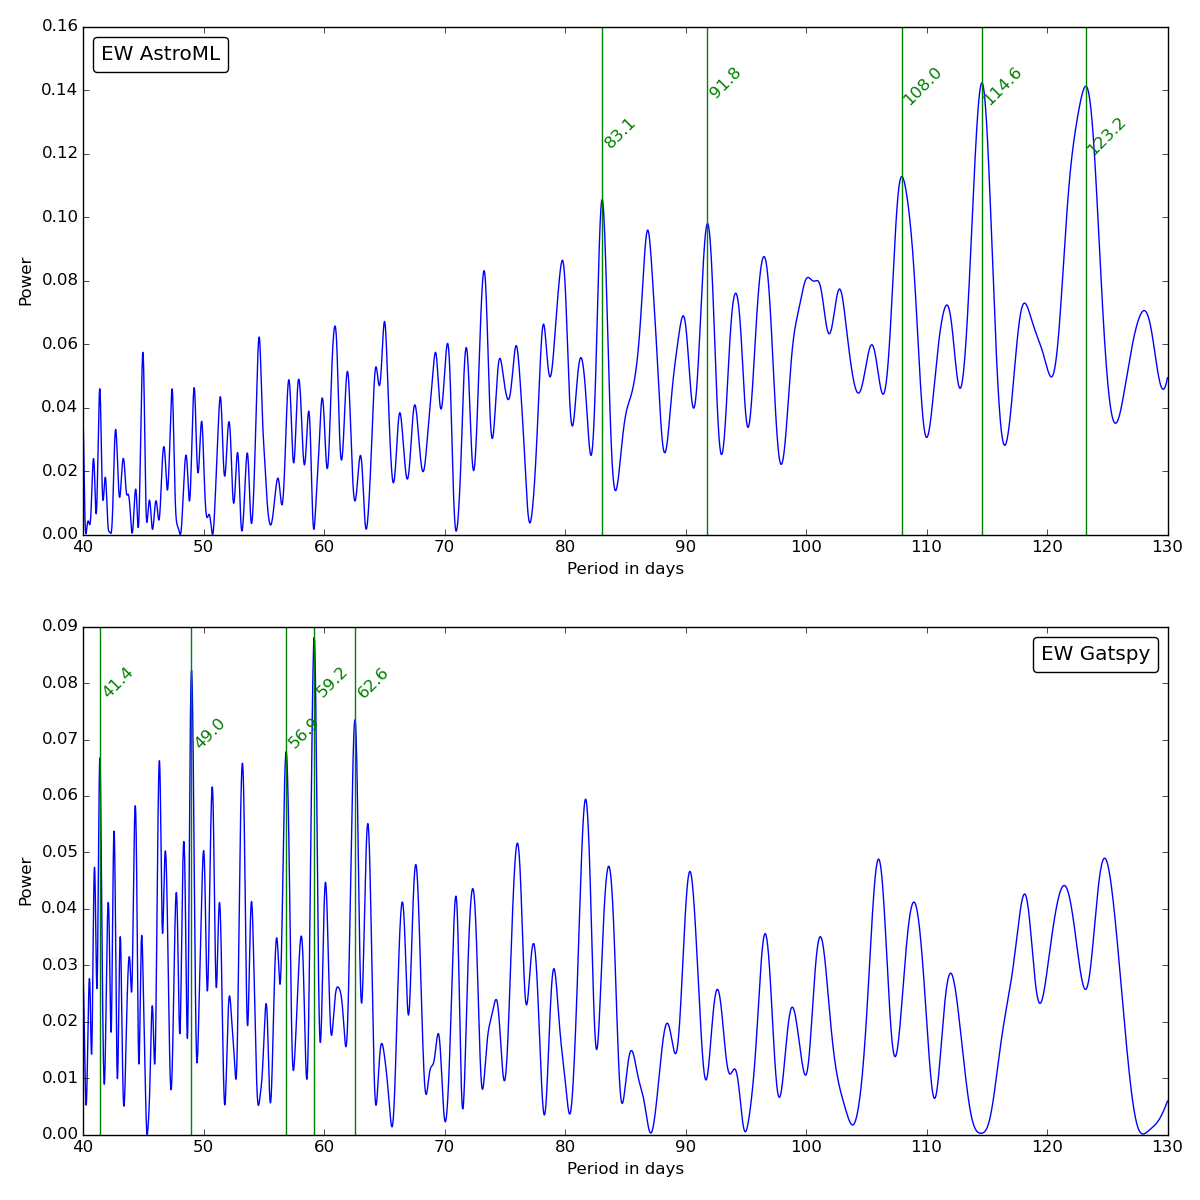
\includegraphics[scale=0.20]{Figures/summpgrams.png} \\
\end{center}   
\caption{This figure shows sample periodograms from the {\ha} peak of the {\harps} data, calculating from Equivalent
  Widths using {\astroml} for the upper panel and {\gatspy} for the lower panel. This corresponds to the second and
  third rows of Table \ref{table:fullewtaball}. The strongest 5 peaks are highlighted in both cases.}
\protect\label{fig:harpspgrams1}
\end{figure}

\begin{figure}[!htbp]
\begin{center}
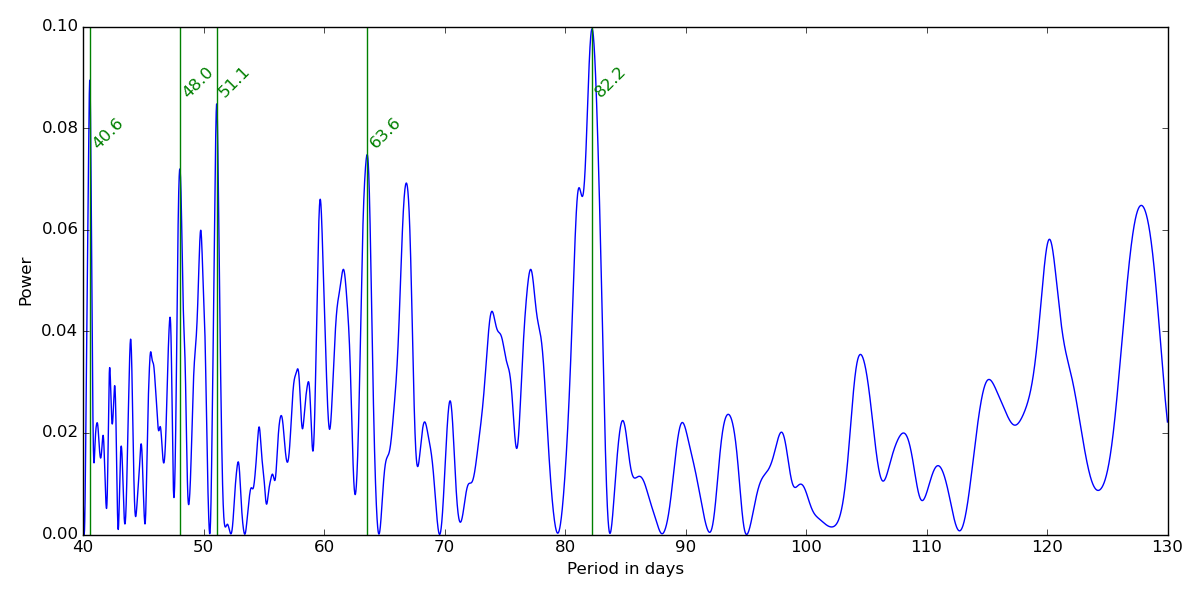
\includegraphics[scale=0.40]{Figures/harpsprbind1.png} \\
\end{center}   
\caption{This figure shows a sample periodogram from the Peak Ratio measure from the Full Set of the data from {\harps}
  binned to 1 day, processed by the {\gatspy} routine and displayed with the five highest peaks highlighted and showing
  the values. This corresponds to the ninth row Table \ref{table:fullprtaball}.}
\protect\label{fig:harpspgrams2}
\end{figure}

Some efforts were made to remove data contaminated from flares, either by clipping spectra with various upper bounds of
Equivalent Width, by binning data or both. Following the lead from {\uves} in Section \ref{section:uvesflares}, spectra
were clipped where the Equivalent Width exceeded one standard deviation from the median. This was 3.8 for the Original
Set or 4.2 for the Full Set of data. However the latter, which included some spectra with very large equivalent widths
taken in 2016, did not yield any particular benefit, so with the full set of data, clipping to a maximum Equivalent
Width of 3.8 in line with the Original Set was tried. Binning to 1 day was attempted as was binning to 0.5 days. In
terms of effectiveness 

The results from the {\ha} Index were almost identical to those from the Equivalent Width measure, so in the majority of
the tables the latter is focused upon, together with Peak Ratios, Skewness and Kurtosis. The full results for these are
found in Appendix \ref{chapter:pgramdetail} and tables \ref{table:origewtaball}, \ref{table:fullewtaball},
\ref{table:origprtaball}, \ref{table:fullprtaball}, \ref{table:origskewtaball}, \ref{table:fullskewtaball},
\ref{table:origkurttaball} and \ref{table:fullkurttaball}. In Table \ref{table:perftable} below these tables in Appendix
\ref{chapter:pgramdetail} are summarised by summarising the occurrences of 82.6 days in the first five peaks within 0.5\%
and 2\% and either 82.6 or the half-period of 41.3 days to the same percentages.

\begin{table}[!htbp]
\centering
\scalebox{0.75}{
\begin{tabular}{|l|l|r|r|r|r|}
\hline
\textbf{Measure}&\textbf{Data set}&\multicolumn{2}{|c|}{\textbf{82.6 days}}&\multicolumn{2}{|c|}{\textbf{82.6 or 41.3 days}}\\\hline
&&\textbf{Up to 0.5\%}&\textbf{Up to 2\%}&\textbf{Up to 0.5\%}&\textbf{Up to 2\%}\\\hline
\multirow{2}{*}{Peak Ratio}&Original&38 & 62 & 48 & 76\\
&Full&47 & 53 & 47 & 60\\\hline
\multirow{2}{*}{Equivalent Width}&Original& 5 & 5 & 43 & 43\\
&Full&3 & 57 & 30 & 83\\\hline
\multirow{2}{*}{Skewness}&Original&0 & 24 & 0 & 24\\
&Full&0 & 40 & 10 & 50\\\hline
\multirow{2}{*}{Kurtosis}&Original&0 & 29 & 0 & 29\\
&Full&17 & 27 & 17 & 27\\\hline
\end{tabular}}
\caption{This table summarises the approximate recovery performance in terms of finding the expected period of 82.6 and
  this or the half-period of 41.3 within the first five peaks and within a given percentage considering all line measurement methods employed with the
  original and full data. All clipping and binning of the data is included in the summary for each method. The full data
  is listed in Appendix \ref{chapter:pgramdetail}.}
\protect\label{table:perftable}
\end{table}

Also examined was the peak for TiO peak highlighted in Fig. \ref{fig:harpsfirstha}, right panel and shown in larger
scale in Fig. \ref{fig:tispec}. Results are presented in Table \ref{table:tipeakall} in Appendix \ref{chapter:pgramdetail}.
However no trace of the 82.6 day period was seen in the results from this, although there were some hints of the 106 day
period noticed in the {\asas} results in Section \ref{section:asas}. Attempts to combine this with the {\ha} peak to
derive a type of a composite spectral index as discussed in \citet{hall99} and \citet{hall00} proved of little value as
the {\ha] peak is so much greater and the results were indistinguishable from the {\ha} results alone.

Again as with the {\asas} and {\hst} data, after checking for other periodic signals of up to the span of the data, it
was not possible to discern any strong period and in particular no sign of the 442-day period reported in
\citet{cincunegui07}.
